\documentclass{article}

\usepackage{style}


\usepackage{Sweave}
\begin{document}

\Sconcordance{concordance:can_we_do_it.tex:can_we_do_it.Rnw:%
1 5 1 1 0 185 1}


\vspace{20mm}


\begin{Large}
\begin{center}
Background and research protocol
\end{center}
\end{Large}


\begin{large}
\begin{center}
\textbf{Can we do it? A survey of research professionals on the timeline and obstacles to eliminating malaria} 
\end{center}
\end{large}


\vspace{5mm}

\begin{changemargin}{2.5cm}{2.5cm} 
\begin{center}
\begin{large}
Joe Brew \hfill \emph{joe.brew@isglobal.org} \\
Elisa Sicuri \hfill \emph{elisa.sicuri@isglobal.org} \\ 
\end{large}
\end{center}
\end{changemargin}


\vspace{6mm}

\begin{center}
\begin{large}
Institut de Salut Global de Barcelona 
\end{large}
\end{center}


\begin{changemargin}{3cm}{3cm} 

\begin{center}
\textbf{Summary}
\end{center}

\emph{In recent years, much of the discourse regarding malaria has shifted from "control" to "eradication." The emphasis on elimination serves to rally funder support, motivate researchers, and focus the efforts of public health practitioners. Proponents of disease eradication point to the success of historical and current campaigns (smallpox and polio, respectively), and highlight the benefits in health and wealth to future generations. However, the opportunity cost of investments in eradication-specific interventions is high, and the expected value of these interventions is a function of thir lag and likelihood of success. In a systematic survey of experts in the field of malaria, we query beliefs regarding the likelihood and time-frame of eradication, as well as the perceived chief obstacles faced by those striving to eradicate. We assess pessimism/optimism (via the proxy of years-to-eradication), broken down by academic discipline, researcher impact, and years of experience. Our results serve as a barometer of professional opinion, and identify areas of research where experts in the field expect the most resistance.}
\end{changemargin}
\vfill  

\newpage

\section*{Executive summary}

The World Health Organisation's Global Malaria Programme has acknowledged that it "needs to take an official position on how and under what timeline malaria eradication could be achieved" \cite{WHO2015}. Such a position could inform policy, and plays a crucial role in the economic analysis of the expected value of malaria control inteventions. \\

\noindent However, no such position has been taken. Given the inherent incentives working against a realistic assessment of the matter at the individual level (funding prerogatives, political pressure, confirmation bias), the best way to assess the likelihood of and time-frame to malaria eradication is a reliance on the anonymous "wisdom of crowds." Surveying experts, an approach already taken for assessing the time-frame to and chief innovations required for the eradication of some neglected tropical diseases \cite{Keenan2013}, can serve as a useful for barometer for filling measuring professional opinion. \\

\noindent This study proposes to carry out a systematic survey of malaria research professionals from a wide array of academic disciplines in order to estimate the likelihood of and time-frame to malaria eradication. Its results can serve as a barometer of professional opinion, informing policy and guiding resources.



\section*{Structure}

This document is divided into three sections:
\vspace{-3mm}

\begin{enumerate}
  \setlength\itemsep{-0.5em}
\item A background, which provides a justification for the proposal and situates this research within the relevant literature, while also outlining the history and current "état de l'art" of global discourse on malaria control and eradication
\item A proposed protocol for review by and approval of the ISGlobal scientific committee
\item Hypothetical examples of visual "knowledge products" to be generated from this research
\end{enumerate}



\vspace{5mm}

\tableofcontents


\newpage  
\section*{Part 1: Background}
\addcontentsline{toc}{section}{Part 1: Background}


\subsection*{Context}
\addcontentsline{toc}{subsection}{Context}

In recent years, researchers, public health agencies and funding organizations have become increasingly interested in transitioning from an approach of malaria "control" to one of "elimination" and "eradication" \cite{Tanner2015}. Even in areas of high endemicity, advances in immunology, parasitology, modeling and vaccinology, along with rapid economic development, have made eradication appear a more feasible goal, even if not possible in the immediate short term \cite{Snow2015, Eckhoff2014}.  \\


\subsection*{Justification}
\addcontentsline{toc}{subsection}{Justification}


\noindent The economic case for striving to achieve malaria eradication is compelling \cite{Barofsky2015}. Though the case-specific marginal cost of prevention can be expected to be high (relative to a simple control approach), successful eradication would mean massive recurring savings in the long-term. However, to the extent that the case-specific marginal cost of prevention in an eradication campaign is high, estimating the likelihood of success is fundamental to the correct distribution of resources, particularly in low-income environments. \\

\noindent In other words, the rational assignment of resources for malaria eradication campaigns hinges on the expected value of those campaigns. We can describe this relationship formulaically below: 

\begin{center}
% 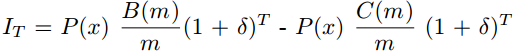
\includegraphics[width=3in]{formula.png}
$I_{T}$ = $P(x)_{}$ $\dfrac{B(m_{})}{m_{}}$(1 + $\delta$)$^{T}$ -  $P(x)_{}$ $\dfrac{C(m_{})}{m_{}}$ (1 + $\delta$)$^{T}$
\end{center}

\noindent Where:
\begin{itemize}
\item $ I $ is the return on investment
\item $ m $ is the number of malaria cases
\item $ x $ is the cut-off for a "successful campaign", ie the portion of eradication achieved
\item $ T $ is the time-frame 
\item $ P $ is the probability of success
\item $ B $ is the benefit of preventing malaria
\item $ C $ is the cost of preventing malaria
\item $ \delta $ is the discount rate and opportunity cost
\end{itemize}

\noindent $ I $ is the return on investment at time (T) (the "end of malaria"). We take the present value of the benefits multiplied by the probability of succcess minus the value of costs times the probability of success, and multiplyboth terms by the discount rate traised to T to arrive at the return on investment. 

\subsection*{The literature}
\addcontentsline{toc}{subsection}{The literature}


\noindent A great deal of previous research already covers the the cost per case prevented \cite{Sicuri2011, Silumbe2015, Btto2016, IlungaIlunga2014, Dalaba2015}. Likewise, a literature exists which could serve as a model for quantifying the location-specific opportunity costs associated with funneling funds towards malaria eradication \cite{Stuckey2014, White2011, Korenromp2012}. The correct discount rate for estimating the value of future lives saved is more of a philosphical question than an economic one. This leaves only the probability and time-frame to eradication, questions which have been addressed anecdotally, but never answered quantitatively. \\

\noindent The scientific and public health communities have had eradication on their long-term agenda since the World Health Organization established the Global Malaria Eradication Program in the 1950s \cite{Alonso2011, Njera2011}. Following the failure of the WHO's first attempt, the focus shifted away from global eradication and towards local elimination and control strategies. \\


\noindent In the last decade, interest in elimination and eradication has seen a resurgence, as evidenced by the proportion of general research on malaria which pertain to elimination and eradication (below) \footnote{For the purposes of this chart, "general research on malaria" is understood as any article in the PubMed database containing the term "malaria" in either the title or the abstract. Articles which "pertain to elimination and eradication" are understood as any article containing the term malaria as well as either "elimination" or "eradication" in the title or abstract. The search was performed using RISmed package \cite{Kovalchik2015} in R \cite{R}, and the chart was generated with the ggplot2 package \cite{ggplot2}}.

\begin{center}
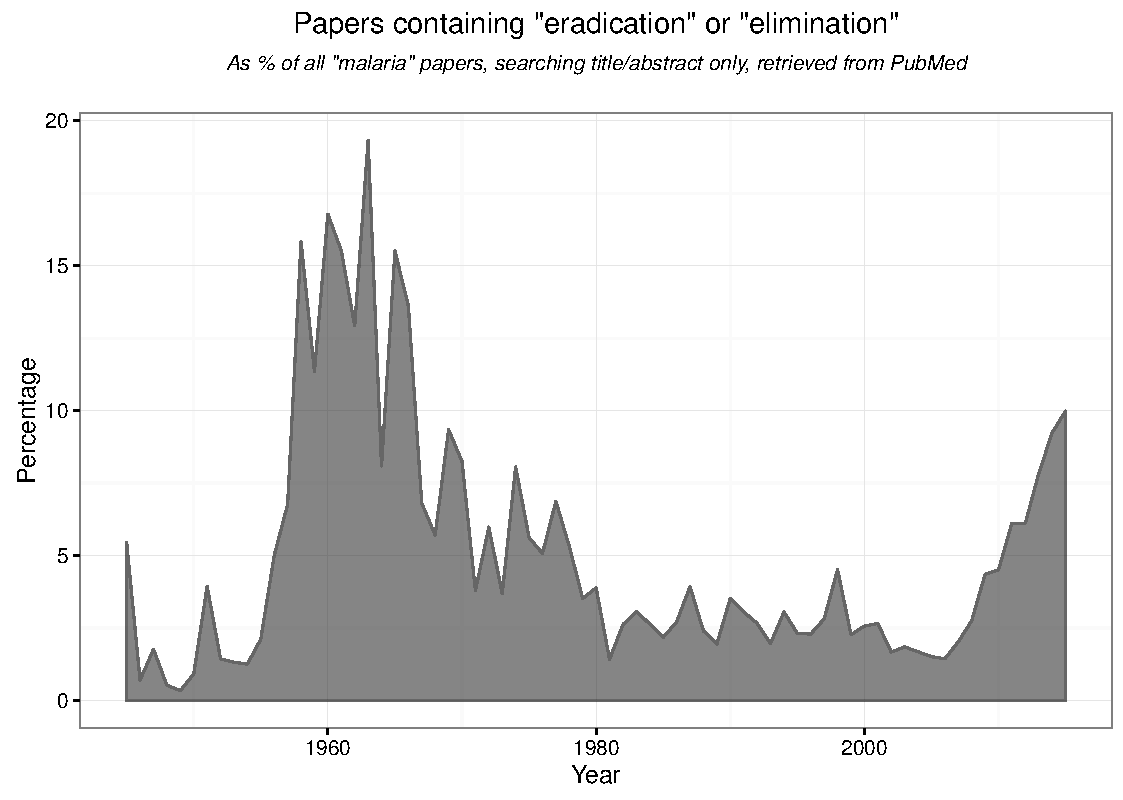
\includegraphics[height=3in]{pubmed2.pdf}
\end{center}


\noindent Most of the current research on expert opinion regarding the feasibility of malaria eradication focuses on the \emph{how} rather than the \emph{if} and the \emph{when} \cite{Tanner2015}. The participants in the Malaria Eradication Research Agenda process, in particular, have positioned themselves as thought leaders in the field of guiding research goals and identifying gaps in order for elmination to occur \cite{Alonso2011}. Though the MalERA authors firmly state that eradication is \emph{not} feasible given the "current tools and state of knowledge", mentions to the time frame are general ("within the lifetime of young scientists just embarking on their careers") and no mention is made of the perception of the probability of achieving eradication.  \\


\noindent In other words, the leaders in the field of malaria have marked a clear path for moving towards eradication, but have not indicated how long walking the path will take. This omission is likely intentional, and certainly understadable, given that MalERA's goals are to guide research and technology in the direction of eradication, and not necessarily address the larger and much more subjective questions of \emph{if} and \emph{when}.  \\

\noindent Though the concept of eradication is often mentioned in both academic and policy circles\cite{Mnzava2014, WHO2016}, the World Health Organisation's Global Malaria Programme (GMP) acknowledges that it "needs to take an official position on how and under what timeline malaria eradication could be achieved" \cite{WHO2015}. However, no official position has been taken.

\subsection*{The need for the wisdom of crowds}
\addcontentsline{toc}{subsection}{The need for the wisdom of crowds}


\noindent Taking an official position is not easy, as it would require the synthesis of learnings from a diversity of fields.   Additionally, taking an official position faces the problem of human bias. Though it's easy to espouse intellectual honesty, leaders and well-known intellectuals in the space of global malaria control face perverse incentives. Funding prerogatives, political pressure and confirmation bias could all potentially serve to "inflate" the stated likelihood of eradication, and "deflate" the stated time-to-eradication. Furthermore, any states forecast exposes itself to the possibility of being incorrect, a reality which encourages stakeholders to embrace generalities and unquantified possibilities. \\


\noindent But quantifying the likelihood of and time-frame to eradication is essential, and far too important to be left o individuals or small panels and committees. It requires the “wisdom of crowds.” Measuring consensus and discord among disease-specific researchers from a variety of disciplines can serve as a barometer of (informed) opinion, both guiding resources and identifying areas of concern. Though the approach is atypical, it is feasible, having previously been undertaken for neglected tropical diseases with a surprisingly high response rate (44\%) \cite{Keenan2013}. \\


\newpage
\section*{Part 2: Protocol}
\addcontentsline{toc}{section}{Part 2: Protocol}


\subsection*{Background}
\addcontentsline{toc}{subsection}{Background}

\noindent \textbf{The wisdom of crowds:} Patients often ask for a “second opinion”, a request which implicitly recognizes two important truths: (1) that an expert can sometimes be wrong and (2) that the combined opinions of multiple experts can better approximate the truth than the opinion of only one. As Sir Francis Galton demonstrated in his famous ox-weight experiment published in Nature1, averaging the opinions of many is more accurate than taking the opinion of any single expert, since the biases of diverse viewpoints can be complementary and symbiotic. \\

\noindent \textbf{The value of forecasting:} In regards to disease eradication, proponents point to the potential ongoing returns on investment to future generations. But economically, the “expected value” of an investment in a binary scenario (eradication or not) is a function of the probability of the scenario’s occurrence, and the temporal lag of that occurrence. Therefore, knowing the likelihood and time-frame of eradication of malaria is essential for making sound investments in health. \\

\noindent \textbf{Why this study:} Assessing likelihood and time-frame of eradication is too important of a task to be left to individuals or small panels and committees. It requires the “wisdom of crowds.” Measuring consensus and discord among disease-specific researchers from a variety of disciplines can serve as a barometer of (informed) opinion, both guiding resources and identifying areas of concern.

\subsection*{Objectives}
\addcontentsline{toc}{subsection}{Objectives}


In a systematic survey of experts in the fields of malaria, we will query perceptions regarding the feasibility and time-frame of eradication, as well as the perceived gaps and chief areas that need attention in order for eradication to occur. We will report on aggregate results, and our analysis will be broken down by disease, researcher academic discipline, impact and years of experience. \\


\noindent Our principal objective is to measure the perceived likelihood/feasibility and time-frame of eradication of malaria among those who are professional researchers of those respective diseases, at a larger scale than any previous study. Our secondary objective is to examine the relationship between the perceived likelihood/feasibility of eradication of diseases with the respective attention allotted to them in both the popular and academic literature. Our tertiary objective is to establish which specific areas of knowledge are lacking through an examination of researcher characteristics (academic discipline, geography, etc.) insofar as those characteristics are associated with differential perceptions regarding time-to-eradication.


\subsection*{Methods and Design}
\addcontentsline{toc}{subsection}{Methods and Design}

We will “webscrape” from PubMed the authors, abstracts, and journal information of all articles related to disease X using standardized search terms. We will then send emails to all first, last, and corresponding authors (whose addresses can be located), asking 2 simple questions:  
\begin{enumerate}
\item In your opinion, how many years will it be until disease X is eradicated? (0-99+)
\item Please rank the following ten areas in order of where attention is most needed in order to achieve eradication (10 = attention most needed; 1 = attention least needed).
\end{enumerate}

\noindent These questions can also be answered via an online survey: \href{http://goo.gl/forms/Ib80IwgwQY}{http://goo.gl/forms/Ib80IwgwQY}. \\


\noindent We will then compile a database which links researcher meta-information (percent and number of publications in top-decile journals, publication quantity, geography of institution, geography of research focus, gender, academic discipline) with their surveyed attitudes regarding eradication (years-to-eradication and ordered ranking of factors). \\


\noindent The design of this study is typical, but this study is noteworthy in two areas: (1) its scale (by using automated web-scraping, emailing, and surveying, we will reach the maximum number of experts), and (2) its democratic approach (we assume that the more experts’ opinions reflected, the closer we are to approximating the “truth”). Our results will be of value not only to the scientific community, but also to policy-makers and public health practitioners. By gauging and synthesizing the “wisdom of (informed) crowds”, we aim to establish a barometer of scientific opinion in a manner that is fully reproducible.


\subsection*{Evaluation criteria}
\addcontentsline{toc}{subsection}{Evaluation criteria}


\noindent \textbf{1. What are the ethical considerations that need to be addressed and how will they be addressed?} \\
We will not be collecting personal health information, or any biological samples. Nor will we be dealing in any way, shape or form with health outcomes or treatment data.
We will only contact researchers whose information is publicly available online.   \\

\noindent The only potential area of “sensitive” information pertains to the disclosure of researchers’ opinions. However, we will state clearly in both the “invitation to participate” email as well as in the online survey form that results will be made fully public; researchers who choose not to participate are free to do so, and will not be contacted thereafter.  \\


\noindent \textbf{2. List the ethics committees (both human and/or animal) which either have reviewed or will review this proposal.} \\


\noindent None. Given the nature of this study, no human/animal ethics committees’ review is necessary. \\

\noindent \textbf{3. Describe the expertise required for the project and which member(s) of the research team will provide each area of expertise.} \\


\noindent Area expertise in malaria: Elisa Sicuri and Joe Brew \\
\noindent Area expertise in economic evaluation: Elisa Sicuri \\
\noindent Area expertise in computer-assisted article retrieval and surveying: Joe Brew \\


\noindent \textbf{4. How does the proposal fit in with ISGlobal’s scientific agenda?} \\ 


\noindent ISGlobal is a thought leader in malaria, as well as its corresponding eradication movement. By using modern, technologically-oriented means to establish a “barometer” of international researcher consensus on the perceived feasibility and time-frame of eradication, ISGlobal would cement its position at the center of the ongoing international dialogue on the subject. Furthermore, given ISGlobal’s stake in eradication campaigns, the results of this study could (a) inform which disciplines and diseases have the most “research gaps” to be filled in order to achieve eradication, (b) identify areas of consensus and discord between different disciplines, (c) provide (crowd-informed) estimates of the timeline to eradication. \\

\noindent \textbf{Budget estimation and expected source of funding for this study.} \\

\noindent None. Given that this topic is directly relevant to the PhD-specific research of the researcher (Joe Brew), no project-specific funding is required. \\

\noindent \textbf{Other comments} \\

\noindent Have all co-investigators read and approved this proposal? NO \\
\noindent Do you expect to handle samples of human origin in the study? NO \\
\noindent Do you expect to handle personal information in the study? NO. 

\newpage 
\section*{Part 3: Knowledge products}
\addcontentsline{toc}{section}{Part 3: Knowledge products}

The below are examples of \emph{hypothetical} knowledge products that could emerge from this resarch. \\

\noindent \textbf{Example 1: Distribution of perceptions of years to eradication} \\
\noindent This chart serves as the main “wisdom of crowds” visualization. It shows both the average amount of time experts from different disciplines believe it will take to achieve eradication, while also displaying where there is consensus (as indicated by high peaks) versus discord (as indicated by wide, low peaks). 


\begin{center}
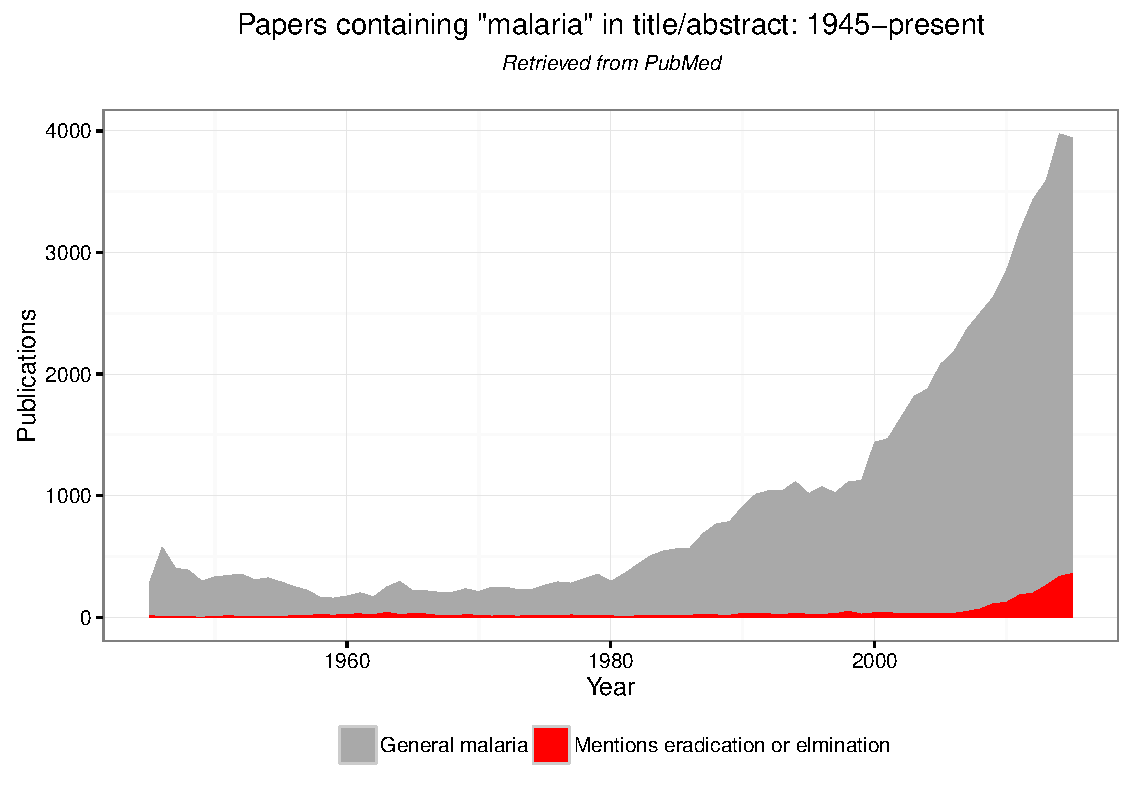
\includegraphics{chart1.pdf}
\end{center}

\newpage
\noindent \textbf{Example 2: The association between researcher “quality” and perception to eradication} \\
\noindent The null hypothesis is that there exists no correlation between the “quality” of a researcher and his/her attitude towards eradication. The alternative hypothesis is that there does exist a correlation. In the case of the alternative hypothesis being validated, this would be evidence that expert opinion should potentially be “weighted” for researcher quality. 

\begin{center}
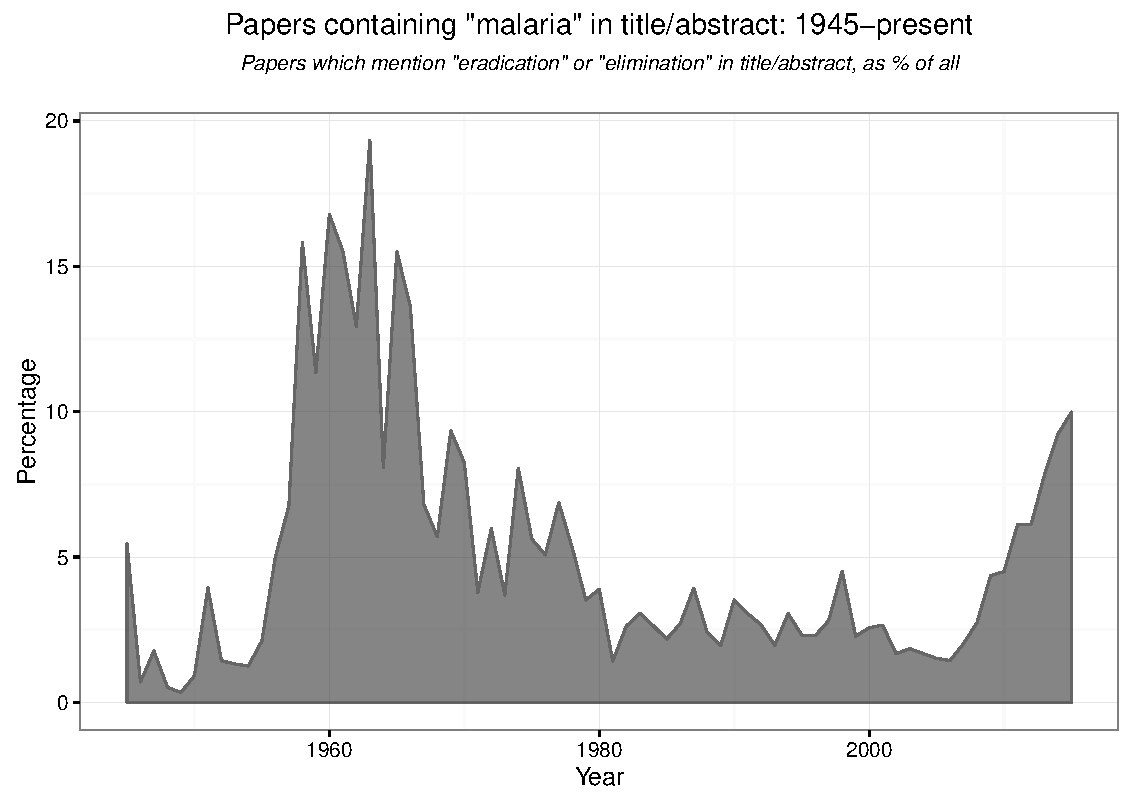
\includegraphics{chart2.pdf}
\end{center}

\newpage
\noindent \textbf{Example 3: Perception of experts of likelihood of short-term eradication by academic discipline} \\
\noindent This chart reveals differential perceptions of the likelihood of short-term eradication by academic discipline. This chart is useful in that if differences are found, this could indicate that disciplines with lower “confidence” in short-term eradication reflect areas that require attention (ie, gaps that need to be filled). For example, if experts from biomedical fields saw high likelihood but experts from anthropology saw low likelihood, this would indicate that the challenges to eradication may be more anthropological than biomedical.

\begin{center}
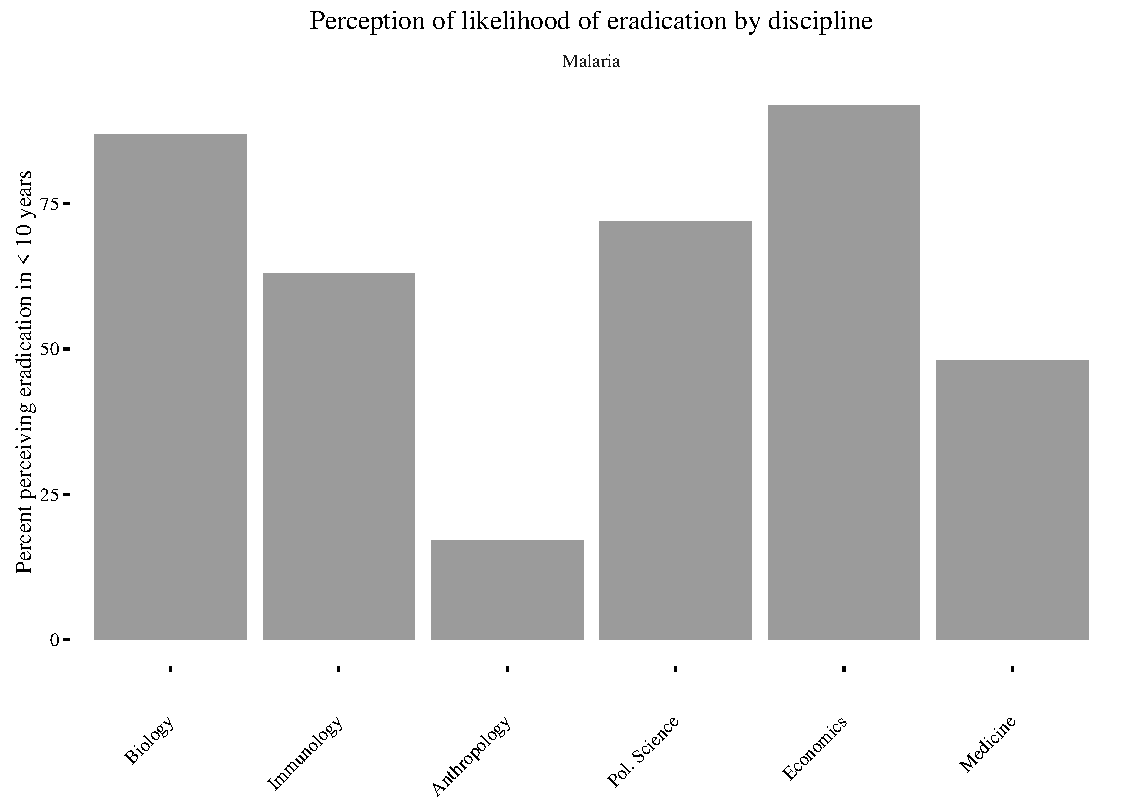
\includegraphics{chart3.pdf}
\end{center}

\newpage
\noindent \textbf{Example 4: Perception of experts regarding area of greatest importance to eradication} \\
\noindent This chart reveals differential perceptions of the area of greatest importance. This chart is useful in that if differences are found, this could indicate that certain areas should receive greatest attention. For example, in the below chart, the highest bar is for “resources for public health”, indicating that (unlike with other NTDs) there is near-consensus among experts that “resources for public health” represents the most important area in order to achieve eradication of malaria

\begin{center}
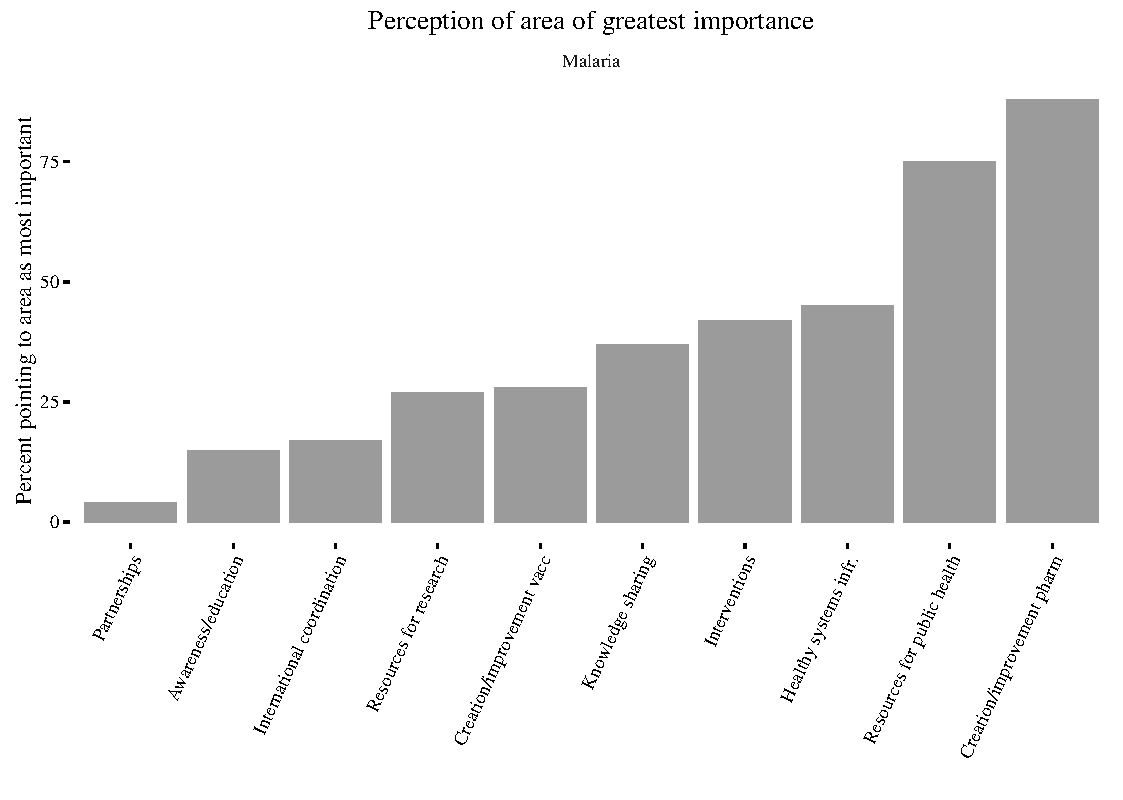
\includegraphics{chart4.pdf}
\end{center}

\newpage
\noindent \textbf{Example 5: Perception of experts regarding area of greatest importance to eradication by academic discipline} \\
\noindent This chart is similar to example 3, but also reflects variation by academic discipline. It indicates how experts of different academic disciplines prioritize different areas of work/research. This is useful in that it indicates the primary concerns of experts from each field, highlighting areas of consensus and discord between diseases and disciplines.

\begin{center}
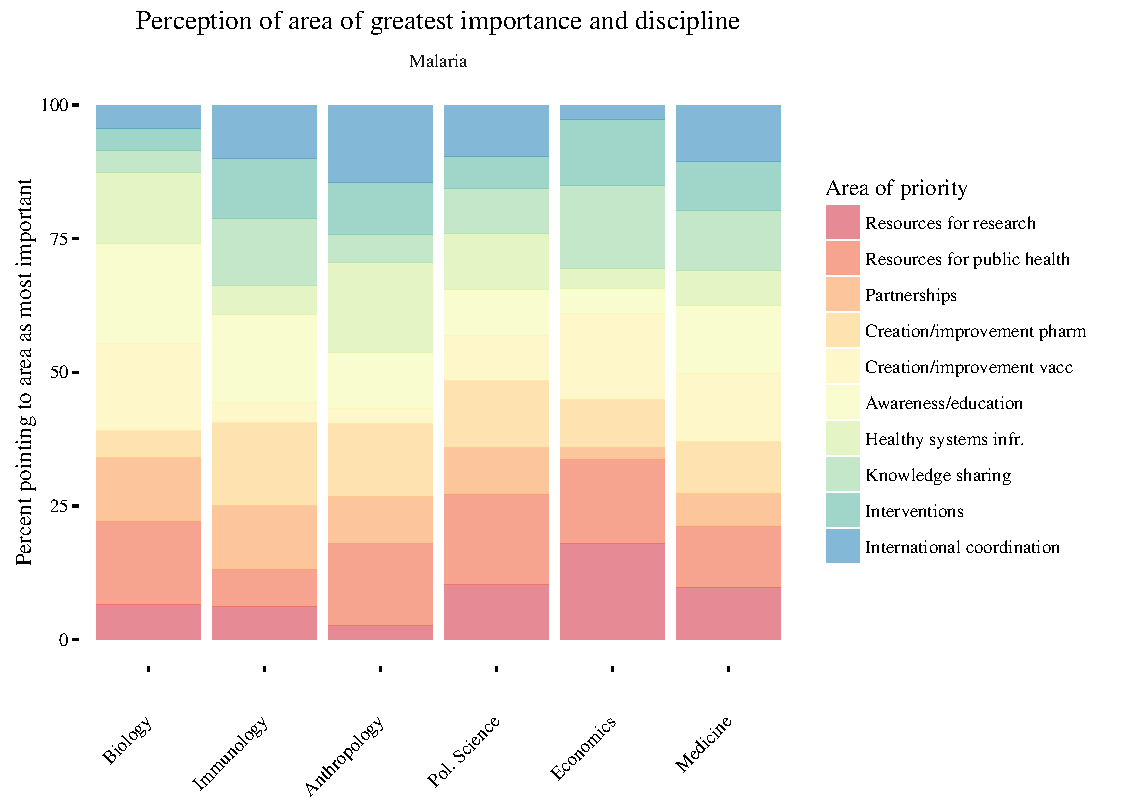
\includegraphics{chart5.pdf}
\end{center}

\newpage

\bibliography{library}{}
\bibliographystyle{apalike}  

\end{document}
